\documentclass[11pt]{article}

    \usepackage[breakable]{tcolorbox}
    \usepackage{parskip} % Stop auto-indenting (to mimic markdown behaviour)
    

    % Basic figure setup, for now with no caption control since it's done
    % automatically by Pandoc (which extracts ![](path) syntax from Markdown).
    \usepackage{graphicx}
    % Maintain compatibility with old templates. Remove in nbconvert 6.0
    \let\Oldincludegraphics\includegraphics
    % Ensure that by default, figures have no caption (until we provide a
    % proper Figure object with a Caption API and a way to capture that
    % in the conversion process - todo).
    \usepackage{caption}
    \DeclareCaptionFormat{nocaption}{}
    \captionsetup{format=nocaption,aboveskip=0pt,belowskip=0pt}

    \usepackage{float}
    \floatplacement{figure}{H} % forces figures to be placed at the correct location
    \usepackage{xcolor} % Allow colors to be defined
    \usepackage{enumerate} % Needed for markdown enumerations to work
    \usepackage{geometry} % Used to adjust the document margins
    \usepackage{amsmath} % Equations
    \usepackage{amssymb} % Equations
    \usepackage{textcomp} % defines textquotesingle
    % Hack from http://tex.stackexchange.com/a/47451/13684:
    \AtBeginDocument{%
        \def\PYZsq{\textquotesingle}% Upright quotes in Pygmentized code
    }
    \usepackage{upquote} % Upright quotes for verbatim code
    \usepackage{eurosym} % defines \euro

    \usepackage{iftex}
    \ifPDFTeX
        \usepackage[T1]{fontenc}
        \IfFileExists{alphabeta.sty}{
              \usepackage{alphabeta}
          }{
              \usepackage[mathletters]{ucs}
              \usepackage[utf8x]{inputenc}
          }
    \else
        \usepackage{fontspec}
        \usepackage{unicode-math}
    \fi

    \usepackage{fancyvrb} % verbatim replacement that allows latex
    \usepackage{grffile} % extends the file name processing of package graphics
                         % to support a larger range
    \makeatletter % fix for old versions of grffile with XeLaTeX
    \@ifpackagelater{grffile}{2019/11/01}
    {
      % Do nothing on new versions
    }
    {
      \def\Gread@@xetex#1{%
        \IfFileExists{"\Gin@base".bb}%
        {\Gread@eps{\Gin@base.bb}}%
        {\Gread@@xetex@aux#1}%
      }
    }
    \makeatother
    \usepackage[Export]{adjustbox} % Used to constrain images to a maximum size
    \adjustboxset{max size={0.9\linewidth}{0.9\paperheight}}

    % The hyperref package gives us a pdf with properly built
    % internal navigation ('pdf bookmarks' for the table of contents,
    % internal cross-reference links, web links for URLs, etc.)
    \usepackage{hyperref}
    % The default LaTeX title has an obnoxious amount of whitespace. By default,
    % titling removes some of it. It also provides customization options.
    \usepackage{titling}
    \usepackage{longtable} % longtable support required by pandoc >1.10
    \usepackage{booktabs}  % table support for pandoc > 1.12.2
    \usepackage{array}     % table support for pandoc >= 2.11.3
    \usepackage{calc}      % table minipage width calculation for pandoc >= 2.11.1
    \usepackage[inline]{enumitem} % IRkernel/repr support (it uses the enumerate* environment)
    \usepackage[normalem]{ulem} % ulem is needed to support strikethroughs (\sout)
                                % normalem makes italics be italics, not underlines
    \usepackage{soul}      % strikethrough (\st) support for pandoc >= 3.0.0
    \usepackage{mathrsfs}
    

    
    % Colors for the hyperref package
    \definecolor{urlcolor}{rgb}{0,.145,.698}
    \definecolor{linkcolor}{rgb}{.71,0.21,0.01}
    \definecolor{citecolor}{rgb}{.12,.54,.11}

    % ANSI colors
    \definecolor{ansi-black}{HTML}{3E424D}
    \definecolor{ansi-black-intense}{HTML}{282C36}
    \definecolor{ansi-red}{HTML}{E75C58}
    \definecolor{ansi-red-intense}{HTML}{B22B31}
    \definecolor{ansi-green}{HTML}{00A250}
    \definecolor{ansi-green-intense}{HTML}{007427}
    \definecolor{ansi-yellow}{HTML}{DDB62B}
    \definecolor{ansi-yellow-intense}{HTML}{B27D12}
    \definecolor{ansi-blue}{HTML}{208FFB}
    \definecolor{ansi-blue-intense}{HTML}{0065CA}
    \definecolor{ansi-magenta}{HTML}{D160C4}
    \definecolor{ansi-magenta-intense}{HTML}{A03196}
    \definecolor{ansi-cyan}{HTML}{60C6C8}
    \definecolor{ansi-cyan-intense}{HTML}{258F8F}
    \definecolor{ansi-white}{HTML}{C5C1B4}
    \definecolor{ansi-white-intense}{HTML}{A1A6B2}
    \definecolor{ansi-default-inverse-fg}{HTML}{FFFFFF}
    \definecolor{ansi-default-inverse-bg}{HTML}{000000}

    % common color for the border for error outputs.
    \definecolor{outerrorbackground}{HTML}{FFDFDF}

    % commands and environments needed by pandoc snippets
    % extracted from the output of `pandoc -s`
    \providecommand{\tightlist}{%
      \setlength{\itemsep}{0pt}\setlength{\parskip}{0pt}}
    \DefineVerbatimEnvironment{Highlighting}{Verbatim}{commandchars=\\\{\}}
    % Add ',fontsize=\small' for more characters per line
    \newenvironment{Shaded}{}{}
    \newcommand{\KeywordTok}[1]{\textcolor[rgb]{0.00,0.44,0.13}{\textbf{{#1}}}}
    \newcommand{\DataTypeTok}[1]{\textcolor[rgb]{0.56,0.13,0.00}{{#1}}}
    \newcommand{\DecValTok}[1]{\textcolor[rgb]{0.25,0.63,0.44}{{#1}}}
    \newcommand{\BaseNTok}[1]{\textcolor[rgb]{0.25,0.63,0.44}{{#1}}}
    \newcommand{\FloatTok}[1]{\textcolor[rgb]{0.25,0.63,0.44}{{#1}}}
    \newcommand{\CharTok}[1]{\textcolor[rgb]{0.25,0.44,0.63}{{#1}}}
    \newcommand{\StringTok}[1]{\textcolor[rgb]{0.25,0.44,0.63}{{#1}}}
    \newcommand{\CommentTok}[1]{\textcolor[rgb]{0.38,0.63,0.69}{\textit{{#1}}}}
    \newcommand{\OtherTok}[1]{\textcolor[rgb]{0.00,0.44,0.13}{{#1}}}
    \newcommand{\AlertTok}[1]{\textcolor[rgb]{1.00,0.00,0.00}{\textbf{{#1}}}}
    \newcommand{\FunctionTok}[1]{\textcolor[rgb]{0.02,0.16,0.49}{{#1}}}
    \newcommand{\RegionMarkerTok}[1]{{#1}}
    \newcommand{\ErrorTok}[1]{\textcolor[rgb]{1.00,0.00,0.00}{\textbf{{#1}}}}
    \newcommand{\NormalTok}[1]{{#1}}

    % Additional commands for more recent versions of Pandoc
    \newcommand{\ConstantTok}[1]{\textcolor[rgb]{0.53,0.00,0.00}{{#1}}}
    \newcommand{\SpecialCharTok}[1]{\textcolor[rgb]{0.25,0.44,0.63}{{#1}}}
    \newcommand{\VerbatimStringTok}[1]{\textcolor[rgb]{0.25,0.44,0.63}{{#1}}}
    \newcommand{\SpecialStringTok}[1]{\textcolor[rgb]{0.73,0.40,0.53}{{#1}}}
    \newcommand{\ImportTok}[1]{{#1}}
    \newcommand{\DocumentationTok}[1]{\textcolor[rgb]{0.73,0.13,0.13}{\textit{{#1}}}}
    \newcommand{\AnnotationTok}[1]{\textcolor[rgb]{0.38,0.63,0.69}{\textbf{\textit{{#1}}}}}
    \newcommand{\CommentVarTok}[1]{\textcolor[rgb]{0.38,0.63,0.69}{\textbf{\textit{{#1}}}}}
    \newcommand{\VariableTok}[1]{\textcolor[rgb]{0.10,0.09,0.49}{{#1}}}
    \newcommand{\ControlFlowTok}[1]{\textcolor[rgb]{0.00,0.44,0.13}{\textbf{{#1}}}}
    \newcommand{\OperatorTok}[1]{\textcolor[rgb]{0.40,0.40,0.40}{{#1}}}
    \newcommand{\BuiltInTok}[1]{{#1}}
    \newcommand{\ExtensionTok}[1]{{#1}}
    \newcommand{\PreprocessorTok}[1]{\textcolor[rgb]{0.74,0.48,0.00}{{#1}}}
    \newcommand{\AttributeTok}[1]{\textcolor[rgb]{0.49,0.56,0.16}{{#1}}}
    \newcommand{\InformationTok}[1]{\textcolor[rgb]{0.38,0.63,0.69}{\textbf{\textit{{#1}}}}}
    \newcommand{\WarningTok}[1]{\textcolor[rgb]{0.38,0.63,0.69}{\textbf{\textit{{#1}}}}}


    % Define a nice break command that doesn't care if a line doesn't already
    % exist.
    \def\br{\hspace*{\fill} \\* }
    % Math Jax compatibility definitions
    \def\gt{>}
    \def\lt{<}
    \let\Oldtex\TeX
    \let\Oldlatex\LaTeX
    \renewcommand{\TeX}{\textrm{\Oldtex}}
    \renewcommand{\LaTeX}{\textrm{\Oldlatex}}
    % Document parameters
    % Document title
    \title{RR\_Project\_Report}
    
    
    
    
    
    
    
% Pygments definitions
\makeatletter
\def\PY@reset{\let\PY@it=\relax \let\PY@bf=\relax%
    \let\PY@ul=\relax \let\PY@tc=\relax%
    \let\PY@bc=\relax \let\PY@ff=\relax}
\def\PY@tok#1{\csname PY@tok@#1\endcsname}
\def\PY@toks#1+{\ifx\relax#1\empty\else%
    \PY@tok{#1}\expandafter\PY@toks\fi}
\def\PY@do#1{\PY@bc{\PY@tc{\PY@ul{%
    \PY@it{\PY@bf{\PY@ff{#1}}}}}}}
\def\PY#1#2{\PY@reset\PY@toks#1+\relax+\PY@do{#2}}

\@namedef{PY@tok@w}{\def\PY@tc##1{\textcolor[rgb]{0.73,0.73,0.73}{##1}}}
\@namedef{PY@tok@c}{\let\PY@it=\textit\def\PY@tc##1{\textcolor[rgb]{0.24,0.48,0.48}{##1}}}
\@namedef{PY@tok@cp}{\def\PY@tc##1{\textcolor[rgb]{0.61,0.40,0.00}{##1}}}
\@namedef{PY@tok@k}{\let\PY@bf=\textbf\def\PY@tc##1{\textcolor[rgb]{0.00,0.50,0.00}{##1}}}
\@namedef{PY@tok@kp}{\def\PY@tc##1{\textcolor[rgb]{0.00,0.50,0.00}{##1}}}
\@namedef{PY@tok@kt}{\def\PY@tc##1{\textcolor[rgb]{0.69,0.00,0.25}{##1}}}
\@namedef{PY@tok@o}{\def\PY@tc##1{\textcolor[rgb]{0.40,0.40,0.40}{##1}}}
\@namedef{PY@tok@ow}{\let\PY@bf=\textbf\def\PY@tc##1{\textcolor[rgb]{0.67,0.13,1.00}{##1}}}
\@namedef{PY@tok@nb}{\def\PY@tc##1{\textcolor[rgb]{0.00,0.50,0.00}{##1}}}
\@namedef{PY@tok@nf}{\def\PY@tc##1{\textcolor[rgb]{0.00,0.00,1.00}{##1}}}
\@namedef{PY@tok@nc}{\let\PY@bf=\textbf\def\PY@tc##1{\textcolor[rgb]{0.00,0.00,1.00}{##1}}}
\@namedef{PY@tok@nn}{\let\PY@bf=\textbf\def\PY@tc##1{\textcolor[rgb]{0.00,0.00,1.00}{##1}}}
\@namedef{PY@tok@ne}{\let\PY@bf=\textbf\def\PY@tc##1{\textcolor[rgb]{0.80,0.25,0.22}{##1}}}
\@namedef{PY@tok@nv}{\def\PY@tc##1{\textcolor[rgb]{0.10,0.09,0.49}{##1}}}
\@namedef{PY@tok@no}{\def\PY@tc##1{\textcolor[rgb]{0.53,0.00,0.00}{##1}}}
\@namedef{PY@tok@nl}{\def\PY@tc##1{\textcolor[rgb]{0.46,0.46,0.00}{##1}}}
\@namedef{PY@tok@ni}{\let\PY@bf=\textbf\def\PY@tc##1{\textcolor[rgb]{0.44,0.44,0.44}{##1}}}
\@namedef{PY@tok@na}{\def\PY@tc##1{\textcolor[rgb]{0.41,0.47,0.13}{##1}}}
\@namedef{PY@tok@nt}{\let\PY@bf=\textbf\def\PY@tc##1{\textcolor[rgb]{0.00,0.50,0.00}{##1}}}
\@namedef{PY@tok@nd}{\def\PY@tc##1{\textcolor[rgb]{0.67,0.13,1.00}{##1}}}
\@namedef{PY@tok@s}{\def\PY@tc##1{\textcolor[rgb]{0.73,0.13,0.13}{##1}}}
\@namedef{PY@tok@sd}{\let\PY@it=\textit\def\PY@tc##1{\textcolor[rgb]{0.73,0.13,0.13}{##1}}}
\@namedef{PY@tok@si}{\let\PY@bf=\textbf\def\PY@tc##1{\textcolor[rgb]{0.64,0.35,0.47}{##1}}}
\@namedef{PY@tok@se}{\let\PY@bf=\textbf\def\PY@tc##1{\textcolor[rgb]{0.67,0.36,0.12}{##1}}}
\@namedef{PY@tok@sr}{\def\PY@tc##1{\textcolor[rgb]{0.64,0.35,0.47}{##1}}}
\@namedef{PY@tok@ss}{\def\PY@tc##1{\textcolor[rgb]{0.10,0.09,0.49}{##1}}}
\@namedef{PY@tok@sx}{\def\PY@tc##1{\textcolor[rgb]{0.00,0.50,0.00}{##1}}}
\@namedef{PY@tok@m}{\def\PY@tc##1{\textcolor[rgb]{0.40,0.40,0.40}{##1}}}
\@namedef{PY@tok@gh}{\let\PY@bf=\textbf\def\PY@tc##1{\textcolor[rgb]{0.00,0.00,0.50}{##1}}}
\@namedef{PY@tok@gu}{\let\PY@bf=\textbf\def\PY@tc##1{\textcolor[rgb]{0.50,0.00,0.50}{##1}}}
\@namedef{PY@tok@gd}{\def\PY@tc##1{\textcolor[rgb]{0.63,0.00,0.00}{##1}}}
\@namedef{PY@tok@gi}{\def\PY@tc##1{\textcolor[rgb]{0.00,0.52,0.00}{##1}}}
\@namedef{PY@tok@gr}{\def\PY@tc##1{\textcolor[rgb]{0.89,0.00,0.00}{##1}}}
\@namedef{PY@tok@ge}{\let\PY@it=\textit}
\@namedef{PY@tok@gs}{\let\PY@bf=\textbf}
\@namedef{PY@tok@ges}{\let\PY@bf=\textbf\let\PY@it=\textit}
\@namedef{PY@tok@gp}{\let\PY@bf=\textbf\def\PY@tc##1{\textcolor[rgb]{0.00,0.00,0.50}{##1}}}
\@namedef{PY@tok@go}{\def\PY@tc##1{\textcolor[rgb]{0.44,0.44,0.44}{##1}}}
\@namedef{PY@tok@gt}{\def\PY@tc##1{\textcolor[rgb]{0.00,0.27,0.87}{##1}}}
\@namedef{PY@tok@err}{\def\PY@bc##1{{\setlength{\fboxsep}{\string -\fboxrule}\fcolorbox[rgb]{1.00,0.00,0.00}{1,1,1}{\strut ##1}}}}
\@namedef{PY@tok@kc}{\let\PY@bf=\textbf\def\PY@tc##1{\textcolor[rgb]{0.00,0.50,0.00}{##1}}}
\@namedef{PY@tok@kd}{\let\PY@bf=\textbf\def\PY@tc##1{\textcolor[rgb]{0.00,0.50,0.00}{##1}}}
\@namedef{PY@tok@kn}{\let\PY@bf=\textbf\def\PY@tc##1{\textcolor[rgb]{0.00,0.50,0.00}{##1}}}
\@namedef{PY@tok@kr}{\let\PY@bf=\textbf\def\PY@tc##1{\textcolor[rgb]{0.00,0.50,0.00}{##1}}}
\@namedef{PY@tok@bp}{\def\PY@tc##1{\textcolor[rgb]{0.00,0.50,0.00}{##1}}}
\@namedef{PY@tok@fm}{\def\PY@tc##1{\textcolor[rgb]{0.00,0.00,1.00}{##1}}}
\@namedef{PY@tok@vc}{\def\PY@tc##1{\textcolor[rgb]{0.10,0.09,0.49}{##1}}}
\@namedef{PY@tok@vg}{\def\PY@tc##1{\textcolor[rgb]{0.10,0.09,0.49}{##1}}}
\@namedef{PY@tok@vi}{\def\PY@tc##1{\textcolor[rgb]{0.10,0.09,0.49}{##1}}}
\@namedef{PY@tok@vm}{\def\PY@tc##1{\textcolor[rgb]{0.10,0.09,0.49}{##1}}}
\@namedef{PY@tok@sa}{\def\PY@tc##1{\textcolor[rgb]{0.73,0.13,0.13}{##1}}}
\@namedef{PY@tok@sb}{\def\PY@tc##1{\textcolor[rgb]{0.73,0.13,0.13}{##1}}}
\@namedef{PY@tok@sc}{\def\PY@tc##1{\textcolor[rgb]{0.73,0.13,0.13}{##1}}}
\@namedef{PY@tok@dl}{\def\PY@tc##1{\textcolor[rgb]{0.73,0.13,0.13}{##1}}}
\@namedef{PY@tok@s2}{\def\PY@tc##1{\textcolor[rgb]{0.73,0.13,0.13}{##1}}}
\@namedef{PY@tok@sh}{\def\PY@tc##1{\textcolor[rgb]{0.73,0.13,0.13}{##1}}}
\@namedef{PY@tok@s1}{\def\PY@tc##1{\textcolor[rgb]{0.73,0.13,0.13}{##1}}}
\@namedef{PY@tok@mb}{\def\PY@tc##1{\textcolor[rgb]{0.40,0.40,0.40}{##1}}}
\@namedef{PY@tok@mf}{\def\PY@tc##1{\textcolor[rgb]{0.40,0.40,0.40}{##1}}}
\@namedef{PY@tok@mh}{\def\PY@tc##1{\textcolor[rgb]{0.40,0.40,0.40}{##1}}}
\@namedef{PY@tok@mi}{\def\PY@tc##1{\textcolor[rgb]{0.40,0.40,0.40}{##1}}}
\@namedef{PY@tok@il}{\def\PY@tc##1{\textcolor[rgb]{0.40,0.40,0.40}{##1}}}
\@namedef{PY@tok@mo}{\def\PY@tc##1{\textcolor[rgb]{0.40,0.40,0.40}{##1}}}
\@namedef{PY@tok@ch}{\let\PY@it=\textit\def\PY@tc##1{\textcolor[rgb]{0.24,0.48,0.48}{##1}}}
\@namedef{PY@tok@cm}{\let\PY@it=\textit\def\PY@tc##1{\textcolor[rgb]{0.24,0.48,0.48}{##1}}}
\@namedef{PY@tok@cpf}{\let\PY@it=\textit\def\PY@tc##1{\textcolor[rgb]{0.24,0.48,0.48}{##1}}}
\@namedef{PY@tok@c1}{\let\PY@it=\textit\def\PY@tc##1{\textcolor[rgb]{0.24,0.48,0.48}{##1}}}
\@namedef{PY@tok@cs}{\let\PY@it=\textit\def\PY@tc##1{\textcolor[rgb]{0.24,0.48,0.48}{##1}}}

\def\PYZbs{\char`\\}
\def\PYZus{\char`\_}
\def\PYZob{\char`\{}
\def\PYZcb{\char`\}}
\def\PYZca{\char`\^}
\def\PYZam{\char`\&}
\def\PYZlt{\char`\<}
\def\PYZgt{\char`\>}
\def\PYZsh{\char`\#}
\def\PYZpc{\char`\%}
\def\PYZdl{\char`\$}
\def\PYZhy{\char`\-}
\def\PYZsq{\char`\'}
\def\PYZdq{\char`\"}
\def\PYZti{\char`\~}
% for compatibility with earlier versions
\def\PYZat{@}
\def\PYZlb{[}
\def\PYZrb{]}
\makeatother


    % For linebreaks inside Verbatim environment from package fancyvrb.
    \makeatletter
        \newbox\Wrappedcontinuationbox
        \newbox\Wrappedvisiblespacebox
        \newcommand*\Wrappedvisiblespace {\textcolor{red}{\textvisiblespace}}
        \newcommand*\Wrappedcontinuationsymbol {\textcolor{red}{\llap{\tiny$\m@th\hookrightarrow$}}}
        \newcommand*\Wrappedcontinuationindent {3ex }
        \newcommand*\Wrappedafterbreak {\kern\Wrappedcontinuationindent\copy\Wrappedcontinuationbox}
        % Take advantage of the already applied Pygments mark-up to insert
        % potential linebreaks for TeX processing.
        %        {, <, #, %, $, ' and ": go to next line.
        %        _, }, ^, &, >, - and ~: stay at end of broken line.
        % Use of \textquotesingle for straight quote.
        \newcommand*\Wrappedbreaksatspecials {%
            \def\PYGZus{\discretionary{\char`\_}{\Wrappedafterbreak}{\char`\_}}%
            \def\PYGZob{\discretionary{}{\Wrappedafterbreak\char`\{}{\char`\{}}%
            \def\PYGZcb{\discretionary{\char`\}}{\Wrappedafterbreak}{\char`\}}}%
            \def\PYGZca{\discretionary{\char`\^}{\Wrappedafterbreak}{\char`\^}}%
            \def\PYGZam{\discretionary{\char`\&}{\Wrappedafterbreak}{\char`\&}}%
            \def\PYGZlt{\discretionary{}{\Wrappedafterbreak\char`\<}{\char`\<}}%
            \def\PYGZgt{\discretionary{\char`\>}{\Wrappedafterbreak}{\char`\>}}%
            \def\PYGZsh{\discretionary{}{\Wrappedafterbreak\char`\#}{\char`\#}}%
            \def\PYGZpc{\discretionary{}{\Wrappedafterbreak\char`\%}{\char`\%}}%
            \def\PYGZdl{\discretionary{}{\Wrappedafterbreak\char`\$}{\char`\$}}%
            \def\PYGZhy{\discretionary{\char`\-}{\Wrappedafterbreak}{\char`\-}}%
            \def\PYGZsq{\discretionary{}{\Wrappedafterbreak\textquotesingle}{\textquotesingle}}%
            \def\PYGZdq{\discretionary{}{\Wrappedafterbreak\char`\"}{\char`\"}}%
            \def\PYGZti{\discretionary{\char`\~}{\Wrappedafterbreak}{\char`\~}}%
        }
        % Some characters . , ; ? ! / are not pygmentized.
        % This macro makes them "active" and they will insert potential linebreaks
        \newcommand*\Wrappedbreaksatpunct {%
            \lccode`\~`\.\lowercase{\def~}{\discretionary{\hbox{\char`\.}}{\Wrappedafterbreak}{\hbox{\char`\.}}}%
            \lccode`\~`\,\lowercase{\def~}{\discretionary{\hbox{\char`\,}}{\Wrappedafterbreak}{\hbox{\char`\,}}}%
            \lccode`\~`\;\lowercase{\def~}{\discretionary{\hbox{\char`\;}}{\Wrappedafterbreak}{\hbox{\char`\;}}}%
            \lccode`\~`\:\lowercase{\def~}{\discretionary{\hbox{\char`\:}}{\Wrappedafterbreak}{\hbox{\char`\:}}}%
            \lccode`\~`\?\lowercase{\def~}{\discretionary{\hbox{\char`\?}}{\Wrappedafterbreak}{\hbox{\char`\?}}}%
            \lccode`\~`\!\lowercase{\def~}{\discretionary{\hbox{\char`\!}}{\Wrappedafterbreak}{\hbox{\char`\!}}}%
            \lccode`\~`\/\lowercase{\def~}{\discretionary{\hbox{\char`\/}}{\Wrappedafterbreak}{\hbox{\char`\/}}}%
            \catcode`\.\active
            \catcode`\,\active
            \catcode`\;\active
            \catcode`\:\active
            \catcode`\?\active
            \catcode`\!\active
            \catcode`\/\active
            \lccode`\~`\~
        }
    \makeatother

    \let\OriginalVerbatim=\Verbatim
    \makeatletter
    \renewcommand{\Verbatim}[1][1]{%
        %\parskip\z@skip
        \sbox\Wrappedcontinuationbox {\Wrappedcontinuationsymbol}%
        \sbox\Wrappedvisiblespacebox {\FV@SetupFont\Wrappedvisiblespace}%
        \def\FancyVerbFormatLine ##1{\hsize\linewidth
            \vtop{\raggedright\hyphenpenalty\z@\exhyphenpenalty\z@
                \doublehyphendemerits\z@\finalhyphendemerits\z@
                \strut ##1\strut}%
        }%
        % If the linebreak is at a space, the latter will be displayed as visible
        % space at end of first line, and a continuation symbol starts next line.
        % Stretch/shrink are however usually zero for typewriter font.
        \def\FV@Space {%
            \nobreak\hskip\z@ plus\fontdimen3\font minus\fontdimen4\font
            \discretionary{\copy\Wrappedvisiblespacebox}{\Wrappedafterbreak}
            {\kern\fontdimen2\font}%
        }%

        % Allow breaks at special characters using \PYG... macros.
        \Wrappedbreaksatspecials
        % Breaks at punctuation characters . , ; ? ! and / need catcode=\active
        \OriginalVerbatim[#1,codes*=\Wrappedbreaksatpunct]%
    }
    \makeatother

    % Exact colors from NB
    \definecolor{incolor}{HTML}{303F9F}
    \definecolor{outcolor}{HTML}{D84315}
    \definecolor{cellborder}{HTML}{CFCFCF}
    \definecolor{cellbackground}{HTML}{F7F7F7}

    % prompt
    \makeatletter
    \newcommand{\boxspacing}{\kern\kvtcb@left@rule\kern\kvtcb@boxsep}
    \makeatother
    \newcommand{\prompt}[4]{
        {\ttfamily\llap{{\color{#2}[#3]:\hspace{3pt}#4}}\vspace{-\baselineskip}}
    }
    

    
    % Prevent overflowing lines due to hard-to-break entities
    \sloppy
    % Setup hyperref package
    \hypersetup{
      breaklinks=true,  % so long urls are correctly broken across lines
      colorlinks=true,
      urlcolor=urlcolor,
      linkcolor=linkcolor,
      citecolor=citecolor,
      }
    % Slightly bigger margins than the latex defaults
    
    \geometry{verbose,tmargin=1in,bmargin=1in,lmargin=1in,rmargin=1in}
    
    

\begin{document}
    
    \maketitle
    
    

    
    \hypertarget{reproducible-research-project}{%
\section{REPRODUCIBLE RESEARCH
PROJECT}\label{reproducible-research-project}}

    June, 2024

    \textbf{Team Members}

\begin{itemize}
\tightlist
\item
  Dominik Koterwa 454845
\item
  Hüseyin Polat 437969
\item
  Nurdan Beşli 457945
\item
  Maciej Lorens 419763
\end{itemize}

    \hypertarget{introduction}{%
\subsection{INTRODUCTION}\label{introduction}}

    Our project is centered on replicating and expanding upon the
groundbreaking machine learning research detailed in the Asian Journal
of Computer and Information Systems (AJCIS), specifically the article
titled `\textbf{Utilisation of Machine Learning Techniques in Testing
and Training of Different Medical Datasets}'. This initiative seeks to
deepen our understanding of how machine learning can revolutionize the
analysis of medical data, thereby enhancing disease detection and
improving diagnostic accuracy across various health conditions.

By engaging with this research, we aim to assess the reproducibility of
the results and explore potential enhancements in the methodology. Our
study will utilize a similar approach to analyze medical datasets,
focusing on maximizing the potential of machine learning in healthcare.
Through rigorous testing and training, our objective is to contribute
meaningful advancements to the medical field, offering insights that
could be vital in developing more effective diagnostic tools and
treatments.

    \hypertarget{datasets}{%
\subsection{DATASETS}\label{datasets}}

    The study we replicated utilized machine learning algorithms to analyze
six different healthcare datasets, all sourced from the \textbf{UC
Irvine Machine Learning Repository}. Each of these datasets varies in
the number of attributes and instances, as detailed below.

    \begin{figure}
\centering
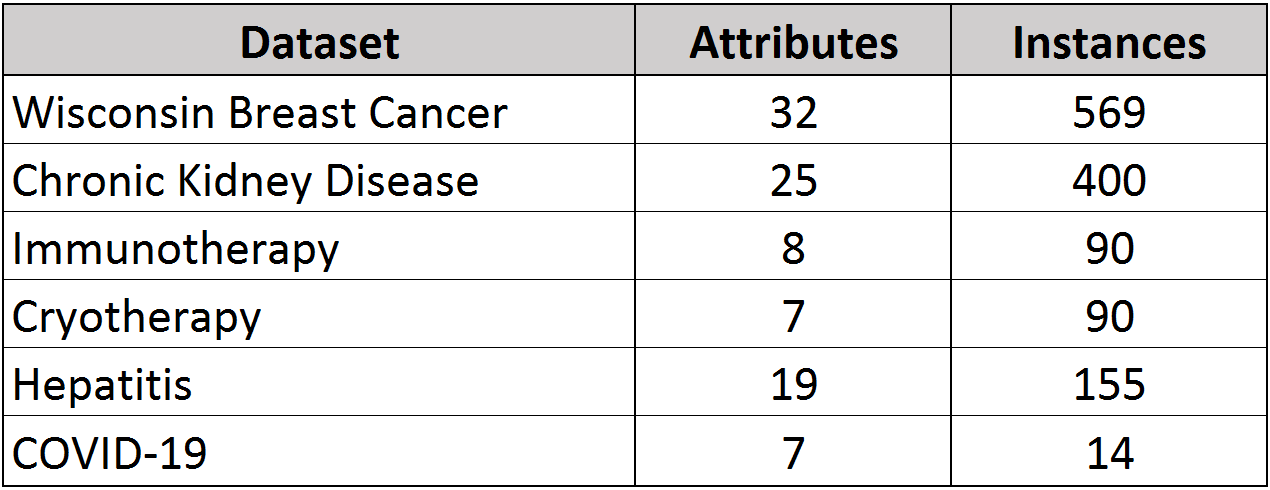
\includegraphics{images/RR_Dataset_Description.PNG}
\caption{RR\_Dataset\_Description}
\end{figure}

    \hypertarget{methodology}{%
\subsection{METHODOLOGY}\label{methodology}}

    \hypertarget{data-preprocessing}{%
\subsubsection{DATA PREPROCESSING}\label{data-preprocessing}}

    For each dataset involved in our study, detailed data preprocessing
steps are applied to ensure compatibility with machine learning models
and to maintain the integrity of the data analysis. Below are the
dataset-specific preprocessing methods implemented:

\textbf{COVID-19 Dataset}

\begin{itemize}
\tightlist
\item
  \textbf{Binary Remapping:} Each categorical variable representing
  binary states (e.g., positive `+' or negative `-') is replaced with
  numerical values where `+' is mapped to 1 and `-' is mapped to 0.
\item
  \textbf{Numerical Conversion:} All columns are converted to numeric
  types to facilitate mathematical operations and model fitting.
\item
  \textbf{Column Renaming:} To clearly indicate the binary nature of the
  data, columns are renamed by adding a `is\_' prefix, enhancing clarity
  and manageability in the dataset.
\end{itemize}

\textbf{Hepatitis Dataset}

\begin{itemize}
\tightlist
\item
  \textbf{Binary Remapping:} Specific columns that contain categorical
  data related to the patient's conditions (e.g., `Steroid',
  `Antivirals', `Fatigue') are converted to binary format, where
  applicable values are adjusted to 0 and 1 to reflect absence and
  presence of the condition.
\item
  \textbf{Mean and Median Imputation:} Missing values are addressed by
  calculating and substituting the mean and median for each column,
  allowing for robustness against outliers and skewed data.
\item
  \textbf{Dropping Missing Data:} Rows containing missing data are
  removed to avoid the introduction of bias or inaccuracies in the
  model's predictions. Corresponding entries in the target variable are
  also excluded to maintain dataset alignment.
\end{itemize}

\textbf{Chronic Kidney Disease Dataset}

\begin{itemize}
\tightlist
\item
  \textbf{Binary Mapping:} Categorical descriptions (e.g., `normal',
  `abnormal'; `present', `notpresent') in symptoms and diagnostic
  results are mapped to binary (1, 0) to simplify the input for
  algorithm processing.
\item
  \textbf{Mean and Median Imputation:} Implements both mean and median
  imputation for handling missing values, providing two sets of data for
  comparative analysis and model robustness.
\item
  \textbf{Dropping Missing Data:} Ensures that only complete data
  entries are processed, by excluding rows with any missing values from
  the analysis, thus maintaining the reliability of the dataset.
\end{itemize}

\textbf{Breast Cancer Dataset}

\begin{itemize}
\tightlist
\item
  \textbf{Binary Mapping:} The target variable `Diagnosis' is converted
  from its original categorical labels (`M' for malignant, `B' for
  benign) into a binary format (1 for malignant, 0 for benign), aligning
  it with binary classification tasks in machine learning.
\item
  \textbf{Data Checks and Cleaning:} Verifies data types, checks for
  outliers, and ensures that all entries are consistent and appropriate
  for analysis.
\end{itemize}

\textbf{Immunotherapy Dataset}

\begin{itemize}
\tightlist
\item
  \textbf{Binary Mapping and Renaming:} Converts `sex' from a
  categorical to a binary format and updates the column name to
  `is\_female' to reflect this binary distinction.
\item
  \textbf{One-Hot Encoding:} Applies one-hot encoding to the `Type'
  column, which involves transforming it into multiple binary columns,
  each representing a different type of immunotherapy, thereby avoiding
  ordinal implications in the categorical data.
\item
  \textbf{Concatenation:} The one-hot encoded columns are then
  concatenated back to the main dataset, preserving the original data
  structure while adding new binary indicators.
\end{itemize}

\textbf{Cryotherapy Dataset}

\begin{itemize}
\tightlist
\item
  \textbf{Binary Mapping:} Converts `sex' to a binary format and adjusts
  column naming similarly to the Immunotherapy dataset to maintain
  consistency.
\item
  \textbf{One-Hot Encoding:} The `Type' column is treated with one-hot
  encoding to convert categorical treatment types into a series of
  binary columns, which are more suitable for machine learning models.
\item
  \textbf{Concatenation of One-Hot Encoded Data:} These binary columns
  are merged back into the primary dataset, ensuring that all data
  remains integrated and accessible for subsequent analysis.
\end{itemize}

    \hypertarget{modeling-and-hyerparameter-optimization}{%
\subsubsection{MODELING AND HYERPARAMETER
OPTIMIZATION}\label{modeling-and-hyerparameter-optimization}}

    In aligning with the methods of the replicated study, we employ the same
machine learning models, each optimized through a systematic
hyperparameter tuning process. The models and their respective
hyperparameters are as follows:

\begin{itemize}
\item
  \textbf{Random Forest (RF):} Optimized for \textbf{n\_estimators} (50,
  100, 200), \textbf{criterion} (`gini', `entropy'), \textbf{max\_depth}
  (None, 10, 20), \textbf{min\_samples\_split} (2, 5, 10),
  \textbf{min\_samples\_leaf} (1, 2, 4), \textbf{max\_features} (`sqrt',
  `log2').
\item
  \textbf{K-Nearest Neighbors (KNN)}: Optimized for
  \textbf{n\_neighbors} (3, 5, 7), \textbf{weights} (`uniform',
  `distance'), \textbf{algorithm} (`auto', `ball\_tree', `kd\_tree',
  `brute'), \textbf{p} (1, 2).
\item
  \textbf{Support Vector Machine (SVM):} Optimized for \textbf{C} (0.1,
  1, 10), \textbf{kernel} (`poly', `rbf'), \textbf{degree} (2, 3).
\item
  \textbf{Decision Tree (DT):} Optimized for \textbf{criterion} (`gini',
  `entropy'), \textbf{splitter} (`best', `random'), \textbf{max\_depth}
  (None, 10, 20), \textbf{min\_samples\_split} (2, 5, 10),
  \textbf{min\_samples\_leaf} (1, 2, 4), \textbf{max\_features} (`sqrt',
  `log2').
\end{itemize}

Hyperparameter tuning is conducted using \textbf{GridSearchCV}, which
incorporates a \textbf{5-fold cross-validation} to ensure robustness and
reliability in model performance. This meticulous optimization process
ensures that each model is finely tuned to provide the best possible
accuracy and generalizability on diverse medical datasets.

    \hypertarget{performance-metrics}{%
\subsubsection{PERFORMANCE METRICS}\label{performance-metrics}}

    In alignment with the replicated study from the Asian Journal of
Computer and Information Systems, we utilize the same performance
metrics to evaluate the effectiveness of the machine learning algorithms
implemented in our research. Each model was applied to the designated
healthcare datasets, and their performance was quantitatively assessed
using the following metrics:

\begin{itemize}
\item
  \textbf{Training Accuracy:} This metric indicates the proportion of
  correct predictions made by the model on the training dataset. It
  provides insight into how well the model learns from the data,
  mirroring the approach taken in the replicated study.
\item
  \textbf{Testing Accuracy:} Reflects the proportion of correct
  predictions on the testing dataset, crucial for understanding how well
  the model generalizes to new, unseen data.
\item
  \textbf{Training Time:} Measures the duration of time the model takes
  to learn from the training data, highlighting the computational
  efficiency of the model during the training phase.
\item
  \textbf{Testing Time:} The time required by the model to make
  predictions on the testing dataset, indicative of the model's
  operational efficiency.
\end{itemize}

Additionally, to further enhance our evaluation framework, we have
incorporated the measurement of the \textbf{Training and Testing F1
Score}, metrics not used in the replicated study. The F1 Score is a
harmonic mean of precision and recall, providing a more nuanced view of
model performance, particularly in the context of imbalanced datasets:

\begin{itemize}
\item
  \textbf{Training F1 Score:} This metric helps assess the balance
  between precision and recall during the model's training phase,
  offering deeper insights into the model's predictive performance and
  accuracy.
\item
  \textbf{Testing F1 Score:} Evaluates the model's precision and recall
  on the testing dataset, which is crucial for applications where the
  cost of false positives and false negatives is significant.
\end{itemize}

By utilizing these metrics, which were also employed in the original
study, we ensure a consistent and comparative approach to evaluating
model performance.

    \hypertarget{results}{%
\subsection{RESULTS}\label{results}}

    \hypertarget{wisconsin-breast-cancer}{%
\subsubsection{Wisconsin Breast Cancer}\label{wisconsin-breast-cancer}}

    \textbf{Training And Testing Time}

    \begin{figure}
\centering
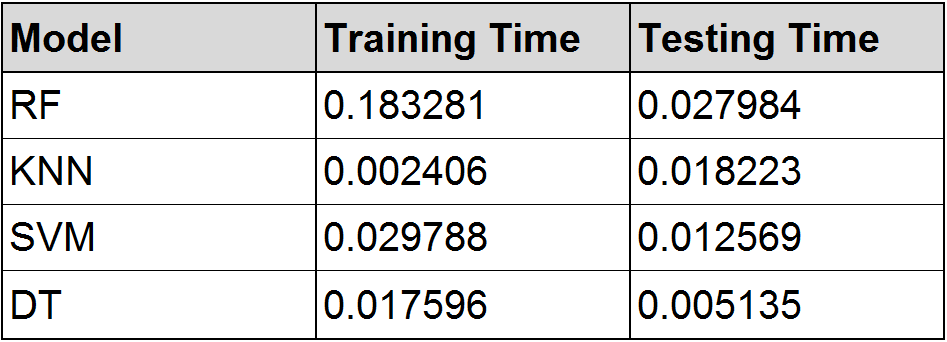
\includegraphics{images/Breast_Cancer_Time.PNG}
\caption{Breast\_Cancer\_Time}
\end{figure}

    \textbf{Accuracy and F1 Score}

    \begin{center}
    \adjustimage{max size={0.9\linewidth}{0.9\paperheight}}{RR_Project_Report_files/RR_Project_Report_22_0.png}
    \end{center}
    { \hspace*{\fill} \\}
    
    \hypertarget{chronic-kidney-disease}{%
\subsubsection{Chronic Kidney Disease}\label{chronic-kidney-disease}}

    \textbf{Training And Testing Time}

    \begin{figure}
\centering
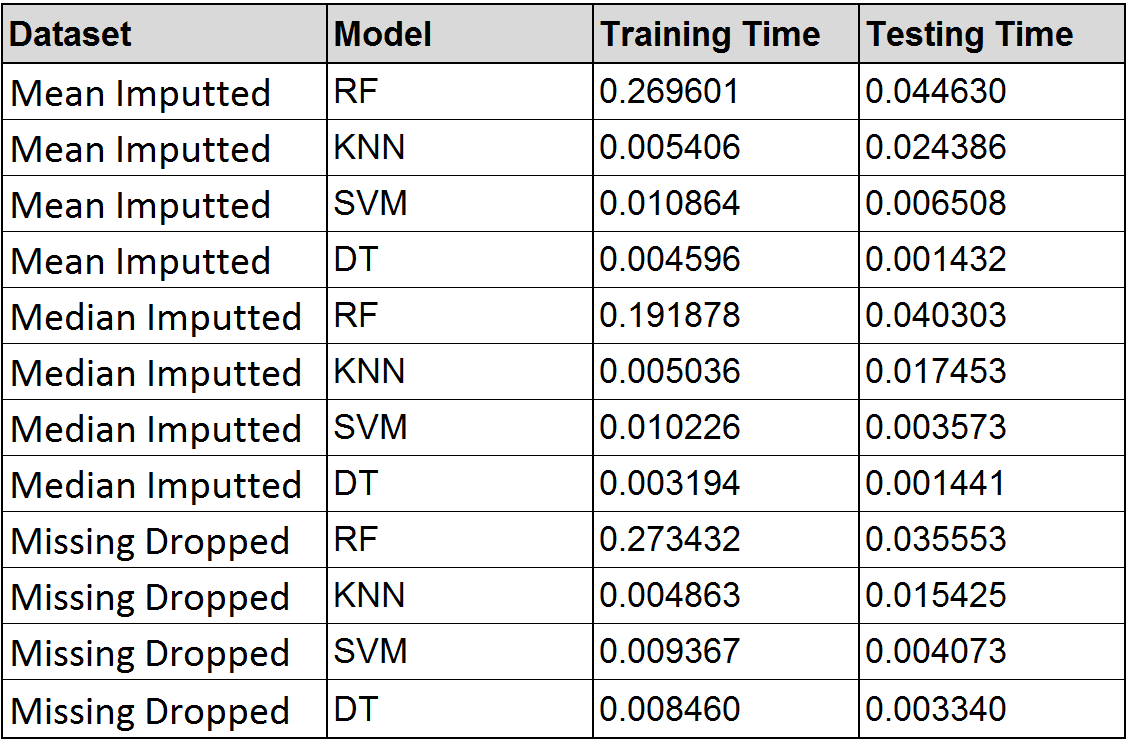
\includegraphics{images/Chronic_Kidney_Disease_Time.PNG}
\caption{Chronic\_Kidney\_Disease\_Time}
\end{figure}

    \textbf{Accuracy and F1 Score}

    \hypertarget{mean-imputted}{%
\subparagraph{Mean Imputted}\label{mean-imputted}}

    \begin{center}
    \adjustimage{max size={0.9\linewidth}{0.9\paperheight}}{RR_Project_Report_files/RR_Project_Report_28_0.png}
    \end{center}
    { \hspace*{\fill} \\}
    
    \hypertarget{median-imputted}{%
\subparagraph{Median Imputted}\label{median-imputted}}

    \begin{center}
    \adjustimage{max size={0.9\linewidth}{0.9\paperheight}}{RR_Project_Report_files/RR_Project_Report_30_0.png}
    \end{center}
    { \hspace*{\fill} \\}
    
    \hypertarget{missing-dropped}{%
\subparagraph{Missing Dropped}\label{missing-dropped}}

    \begin{center}
    \adjustimage{max size={0.9\linewidth}{0.9\paperheight}}{RR_Project_Report_files/RR_Project_Report_32_0.png}
    \end{center}
    { \hspace*{\fill} \\}
    
    \hypertarget{covid-19}{%
\subsubsection{Covid 19}\label{covid-19}}

    \textbf{Training And Testing Time}

    \begin{figure}
\centering
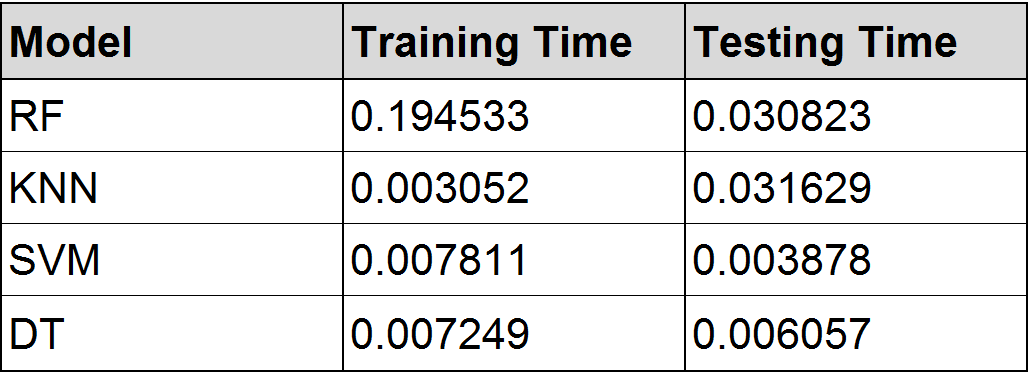
\includegraphics{images/Covid19_Time.PNG}
\caption{Covid19\_Time}
\end{figure}

    \textbf{Accuracy and F1 Score}

    \begin{center}
    \adjustimage{max size={0.9\linewidth}{0.9\paperheight}}{RR_Project_Report_files/RR_Project_Report_37_0.png}
    \end{center}
    { \hspace*{\fill} \\}
    
    \hypertarget{cryotherapy}{%
\subsubsection{Cryotherapy}\label{cryotherapy}}

    \textbf{Training And Testing Time}

    \begin{figure}
\centering
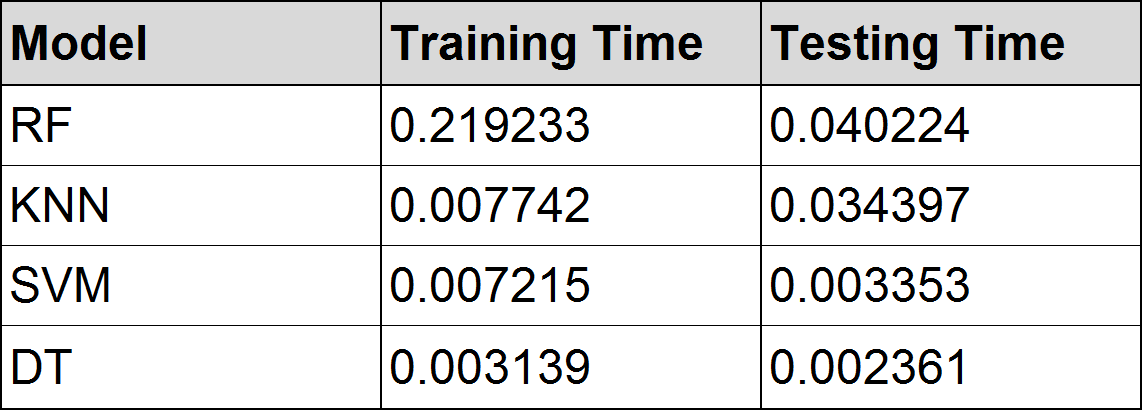
\includegraphics{images/Cryotherapy_Time.PNG}
\caption{Cryotherapy\_Time}
\end{figure}

    \textbf{Accuracy and F1 Score}

    \begin{center}
    \adjustimage{max size={0.9\linewidth}{0.9\paperheight}}{RR_Project_Report_files/RR_Project_Report_42_0.png}
    \end{center}
    { \hspace*{\fill} \\}
    
    \hypertarget{hepatitis}{%
\subsubsection{Hepatitis}\label{hepatitis}}

    \textbf{Training And Testing Time}

    \begin{figure}
\centering
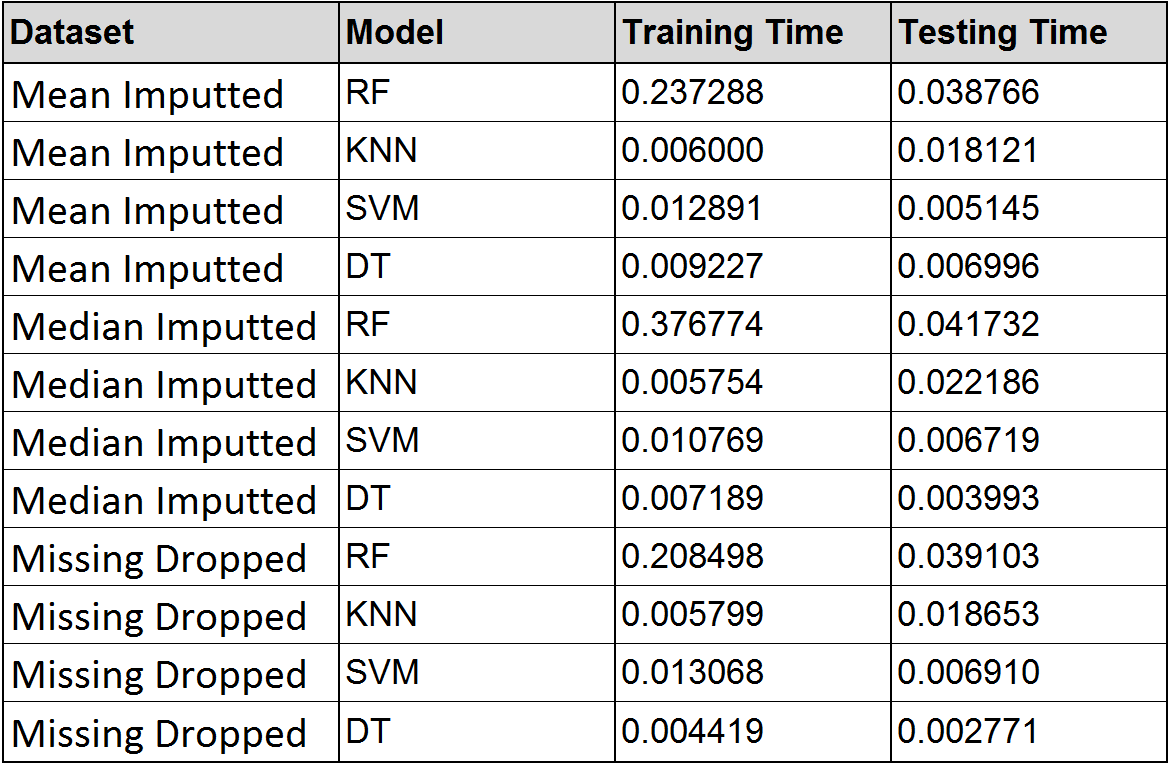
\includegraphics{images/Hepathisis_time.PNG}
\caption{Hepathisis\_time}
\end{figure}

    \textbf{Accuracy and F1 Score}

    \hypertarget{mean-imputted}{%
\subparagraph{Mean Imputted}\label{mean-imputted}}

    \begin{center}
    \adjustimage{max size={0.9\linewidth}{0.9\paperheight}}{RR_Project_Report_files/RR_Project_Report_48_0.png}
    \end{center}
    { \hspace*{\fill} \\}
    
    \hypertarget{median-imputted}{%
\subparagraph{Median Imputted}\label{median-imputted}}

    \begin{center}
    \adjustimage{max size={0.9\linewidth}{0.9\paperheight}}{RR_Project_Report_files/RR_Project_Report_50_0.png}
    \end{center}
    { \hspace*{\fill} \\}
    
    \hypertarget{missing-dropped}{%
\subparagraph{Missing Dropped}\label{missing-dropped}}

    \begin{center}
    \adjustimage{max size={0.9\linewidth}{0.9\paperheight}}{RR_Project_Report_files/RR_Project_Report_52_0.png}
    \end{center}
    { \hspace*{\fill} \\}
    
    \hypertarget{immunotherapy}{%
\subsubsection{Immunotherapy}\label{immunotherapy}}

    \textbf{Training And Testing Time}

    \begin{figure}
\centering
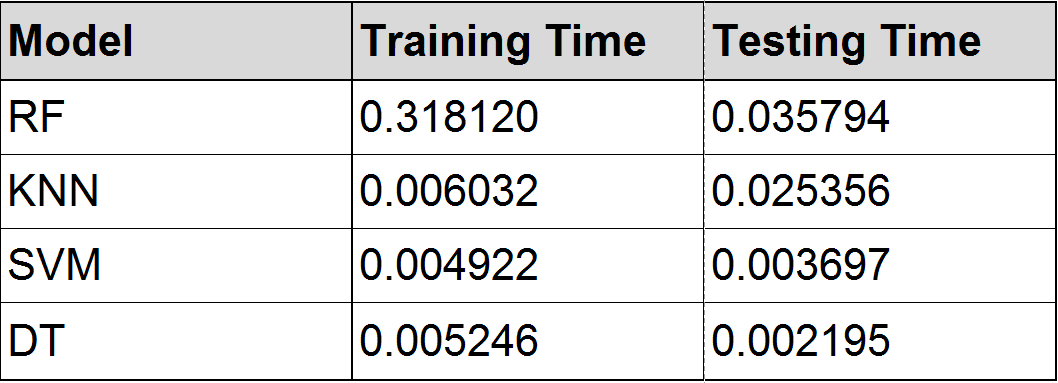
\includegraphics{images/Immunotherapy_time.PNG}
\caption{Immunotherapy\_time}
\end{figure}

    \textbf{Accuracy and F1 Score}

    \begin{center}
    \adjustimage{max size={0.9\linewidth}{0.9\paperheight}}{RR_Project_Report_files/RR_Project_Report_57_0.png}
    \end{center}
    { \hspace*{\fill} \\}
    
    \hypertarget{comparison}{%
\subsection{COMPARISON}\label{comparison}}

    In our replication of the study, we follow the original approach of
categorizing model performance into four levels: \textbf{excellent
execution, good execution, fair execution, and inadequate execution}.
The original study primarily utilizes \textbf{Testing Accuracy} to
compare the performance of models across various datasets, a method we
have also adopted.

In instances where models yield the same Testing Accuracy for the same
datasets, we employ a different approach by further comparing results
using \textbf{Testing F1 Score} and \textbf{Testing Time}. This
adjustment is necessary because, unlike in the original study where all
testing accuracies differed, our replication has encountered scenarios
with identical accuracy scores, necessitating additional metrics for a
comprehensive evaluation.

    \textbf{Our Results Comparison}

    \begin{figure}
\centering
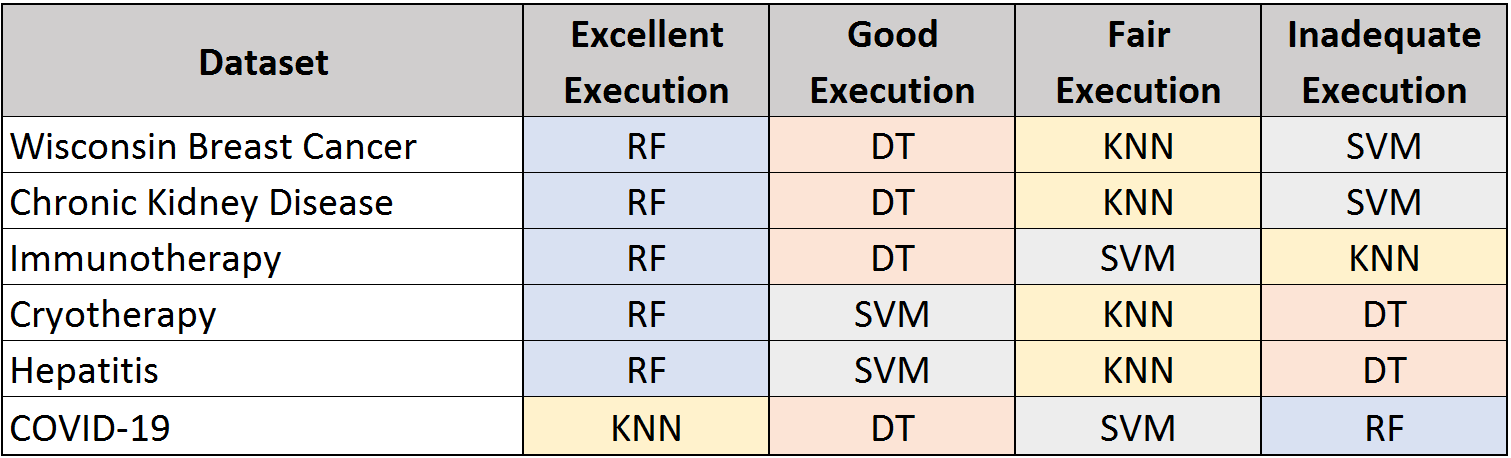
\includegraphics{images/Final_Result_Comparison_Ours.PNG}
\caption{Final\_Result\_Comparison\_Ours}
\end{figure}

    \textbf{Replicated Study Comparison}

    \begin{figure}
\centering
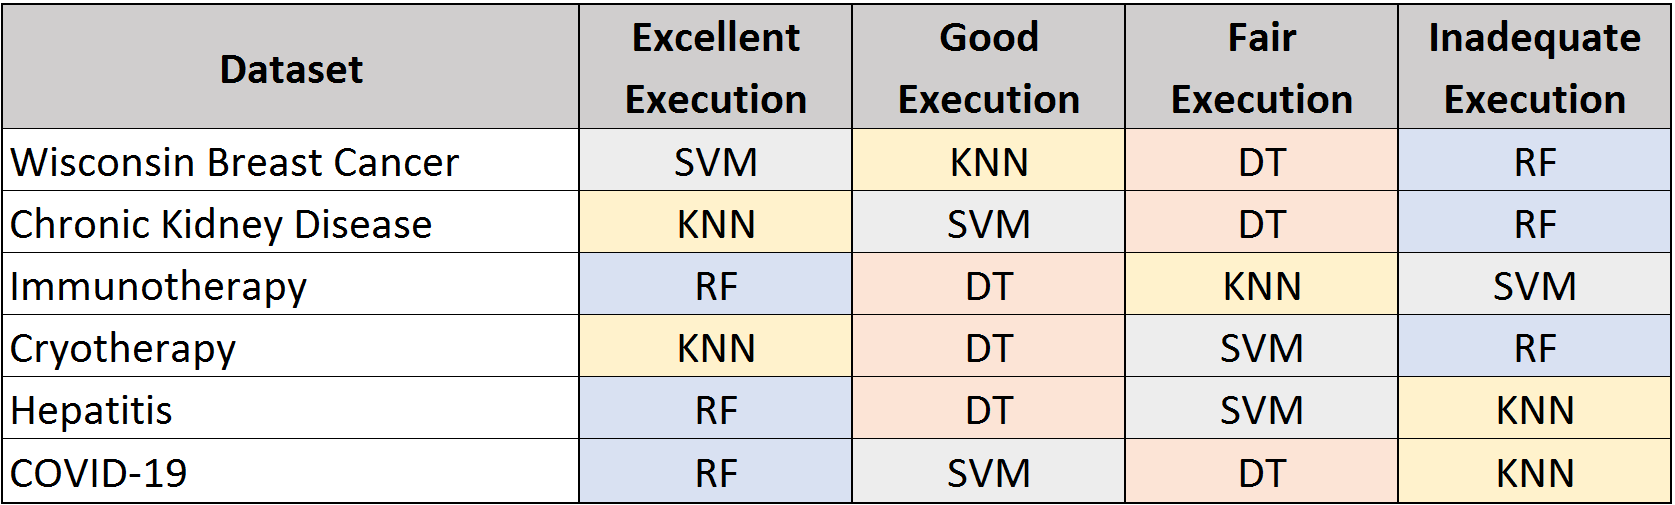
\includegraphics{images/Original_study_comparison.PNG}
\caption{Original\_study\_comparison}
\end{figure}

    Our results exhibit significant differences across almost all datasets
when compared to the replicated study. These variations can primarily be
attributed to the lack of detailed documentation in the replicated study
regarding their methodology, data preprocessing processes, and the
hyperparameters used in the models. In our replication, we employed a
grid search to optimize hyperparameter selection, a method not specified
in the replicated study. Without knowledge of how they chose their
hyperparameters, our reliance on this systematic approach likely
contributed to the observed discrepancies in model performance across
the datasets. This highlights the importance of transparency and
detailed documentation in research to ensure reproducibility and
accurate comparison of results.

    \hypertarget{references}{%
\subsection{REFERENCES}\label{references}}

    \textbf{Replicated Study}

    \begin{itemize}
\tightlist
\item
  Mijwil, M. M., Salem, I. E., \& Abttan, R. A. (2021). Utilisation of
  Machine Learning Techniques in Testing and Training of Different
  Medical Datasets. Asian Journal of Computer and Information Systems,
  9(4), 29. Retrieved from
  https://ajouronline.com/index.php/AJCIS/article/view/6765
\end{itemize}

    \textbf{Datasets}

    All datasets are retrieved from UC Irvine Machine Learning Repository:

\begin{itemize}
\tightlist
\item
  Wisconsin Breast Cancer:
  https://archive.ics.uci.edu/dataset/17/breast+cancer+wisconsin+diagnostic
\item
  Chronic Kidney Disease:
  https://archive.ics.uci.edu/dataset/336/chronic+kidney+disease
\item
  Immunotherapy:
  https://archive.ics.uci.edu/dataset/428/immunotherapy+dataset
\item
  Cryotherapy:
  https://archive.ics.uci.edu/dataset/429/cryotherapy+dataset
\item
  Hepatitis: https://archive.ics.uci.edu/dataset/46/hepatitis
\item
  COVID-19:
  https://archive.ics.uci.edu/dataset/567/covid+19+surveillance
\end{itemize}


    % Add a bibliography block to the postdoc
    
    
    
\end{document}
